% Autor: Francisco Javier Barranco Tena
% Métricas de evaluación utilizadas en el desarrollo del TFG
% Alt + z o Option + z para activar el word wrap en Visual Studio Code

Las métricas de evaluación son una parte fundamental en el desarrollo de modelos de visión por computador. Permiten cuantificar el rendimiento de los modelos y comparar diferentes modelos entre sí. En este TFG se han utilizado varias métricas de evaluación para evaluar los modelos de detección de daños en pavimentos. A continuación, se detallan las métricas de evaluación utilizadas en la CRDDC2022 y en Ultralytics, que son las métricas de evaluación que se han utilizado en los experimentos realizados en este TFG.

\subsubsection{Métricas de evaluación de la CRDDC 2022}
La CRDDC2022 proporciona una métrica de evaluación que se utiliza en los cinco \textit{leaderboards} que han publicado. La CRDDC2022 solo evalúa cinco predicciones por imagen y el resto las ignora. Los modelos se evalúan con F-measure o F1-score. El F1-score se calcula como la media armónica de la precisión y el recall, es decir,
\begin{equation}
    \text{F1} = \frac{2 \cdot Precision \cdot Recall}{Precision + Recall}
\end{equation}

Una predicción se considera correcta si el IoU (Intersección sobre Unión) entre la predicción y el \textit{ground truth} es mayor que 0.5. El IoU se calcula como el área de la intersección entre la predicción y el \textit{ground truth} dividida por el área de la unión entre la predicción y el \textit{ground truth}. La precisión se calcula como el número de predicciones correctas dividido por el número de predicciones totales. El recall se calcula como el número de predicciones correctas dividido por el número de \textit{ground truth}. En la figura \ref{fig:IoU} se puede ver un diagrama que ilustra el cálculo del IoU.

% Añadimos el diagrama de IoU
\begin{figure}[H]
    \centering
    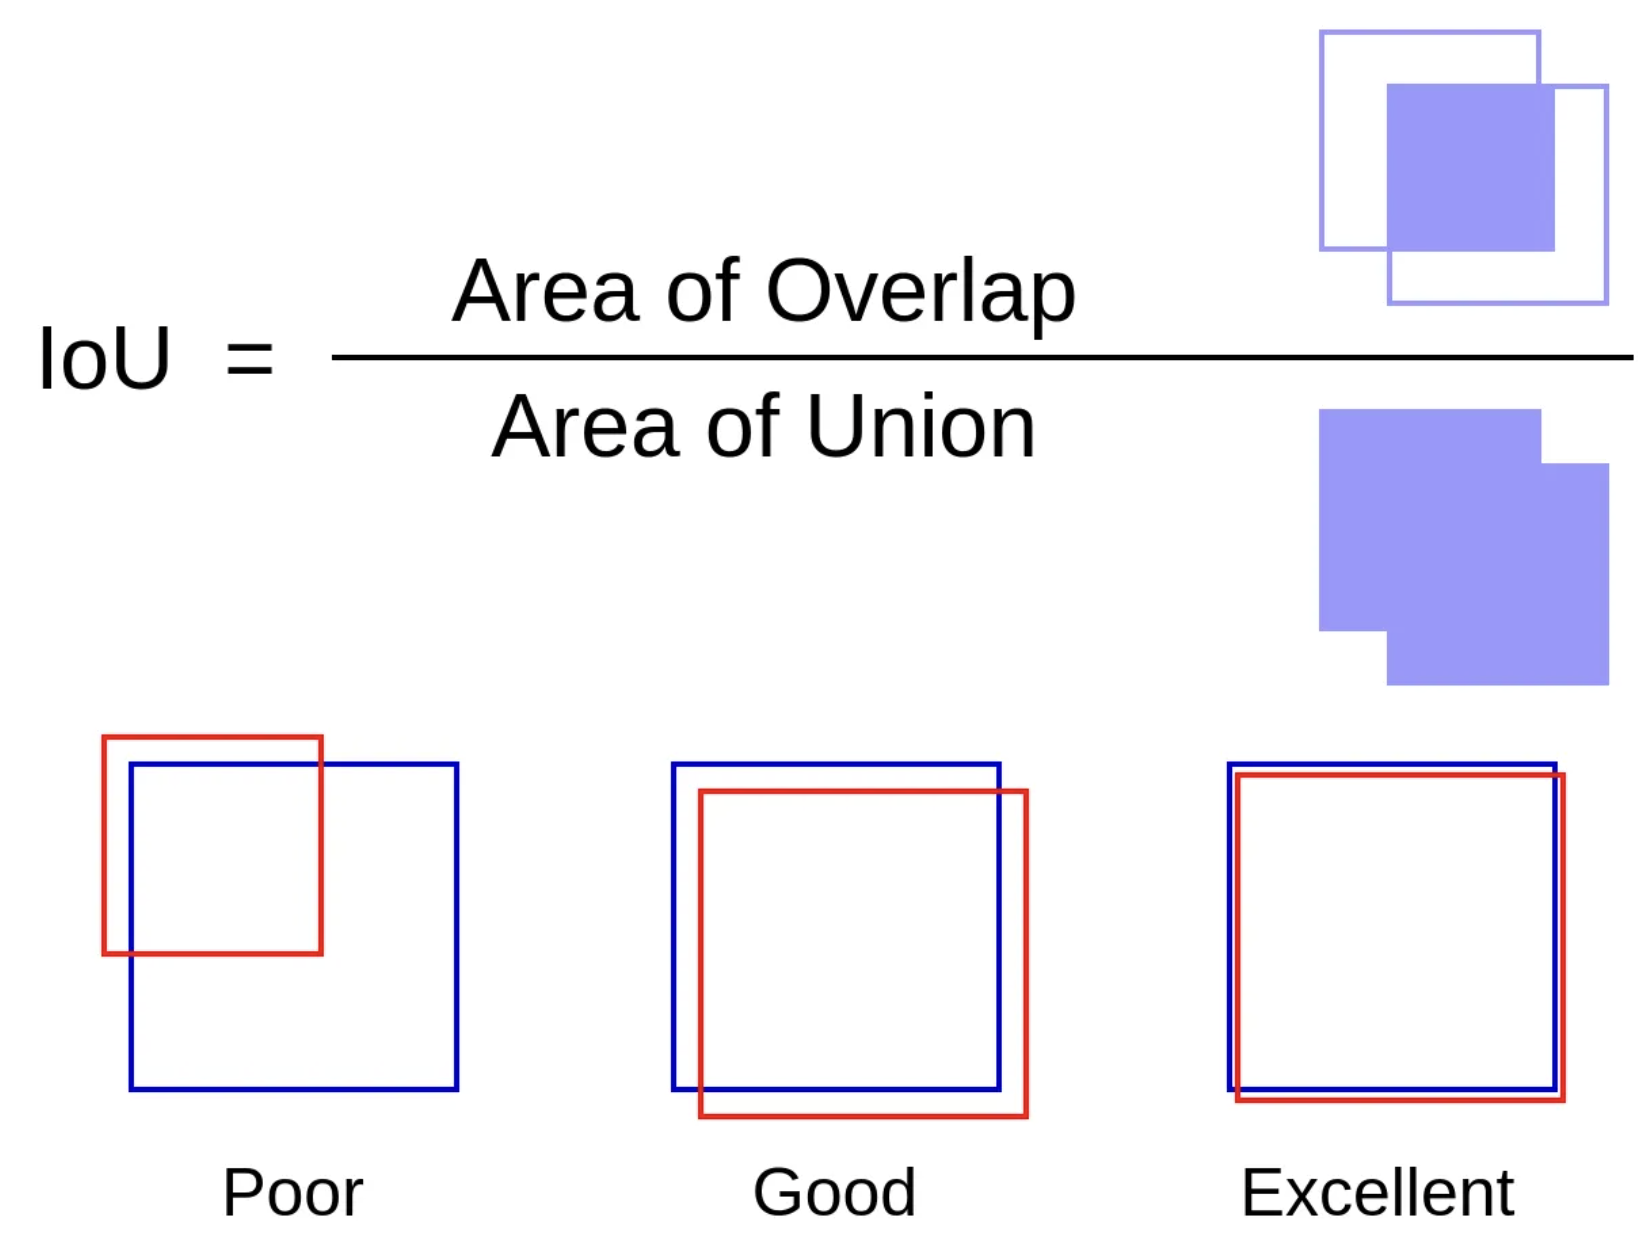
\includegraphics[width=0.4\textwidth]{img/IoU-diagram.png}
    \caption{Diagrama de IoU. \cite{IoU_image}}
    \label{fig:IoU}
\end{figure}

\subsubsection{Métricas de evaluación de Ultralytics\label{SEC:METRICAS_ULTRALYTICS}}
La librería Ultralytics proporciona varias métricas y gráficas que se utilizan para evaluar los modelos de detección de objetos y monitorizar el entrenamiento. Las métricas de evaluación que proporciona Ultralytics son las siguientes:
\begin{itemize}
    \item \textbf{Precisión}: La precisión se calcula como el número de verdaderos positivos dividido por el número de verdaderos positivos más falsos positivos.
    \item \textbf{Recall}: El recall se calcula como el número de verdaderos positivos dividido por el número de verdaderos positivos más falsos negativos.
    \item \textbf{mAP50}: El mAP50 se calcula como el promedio de los AP50 de cada clase. El AP50 se calcula como el área bajo la curva de precisión-recall para un umbral de IoU de 0.5.
    \item \textbf{mAP50-95}: El mAP50-95 se calcula como el promedio de los AP50-95 de cada clase. El AP50-95 se calcula como el área bajo la curva de precisión-recall para un umbral de IoU de 0.5 a 0.95.
    \item \textbf{F1-score}: Ultralytics no proporciona el F1-score directamente, pero se puede calcular a partir de la precisión y el recall como se ha explicado anteriormente.
\end{itemize}

Las gráficas que proporciona Ultralytics son las siguientes (ver figura \ref{fig:Ultralytics_metrics}):

\begin{itemize}
    \item \textbf{Loss curve}: La curva de pérdida muestra la evolución de la pérdida durante el entrenamiento. Permite monitorizar el entrenamiento y detectar posibles problemas como \textit{overfitting}.
    \item \textbf{Matriz de confusión}: La matriz de confusión muestra el número de verdaderos positivos, falsos positivos, verdaderos negativos y falsos negativos para cada clase. Ultralytics genera una versión con valores absolutos y otra con valores normalizados.
    \item \textbf{F1-confidence curve}: La curva F1-confidence muestra el F1-score en función de la confianza de las predicciones. Permite ajustar el umbral de confianza para obtener un F1-score óptimo.
    \item \textbf{Precision-recall curve}: La curva precision-recall muestra la precisión en función del recall para diferentes umbrales de confianza. Permite ajustar el umbral de confianza para obtener un equilibrio entre precisión y recall. También genera las curvas de precision-confidence y recall-confidence.
    \item \textbf{Ejemplos de batch}: Muestra ejemplos de imágenes con las predicciones del modelo. Permite visualizar las predicciones del modelo y compararlas con el \textit{ground truth}.
\end{itemize}

% Añadimos ejemplos de las gráficas de Ultralytics. Tengo metrics_confusion_matrix.png, metrics_PR_curve.png, metrics_results.png y metrics_val_batch0_pred.png. metrics_grid.jpg es una imagen que he creado para mostrar todas las gráficas juntas.
\begin{figure}[H]
    \centering
    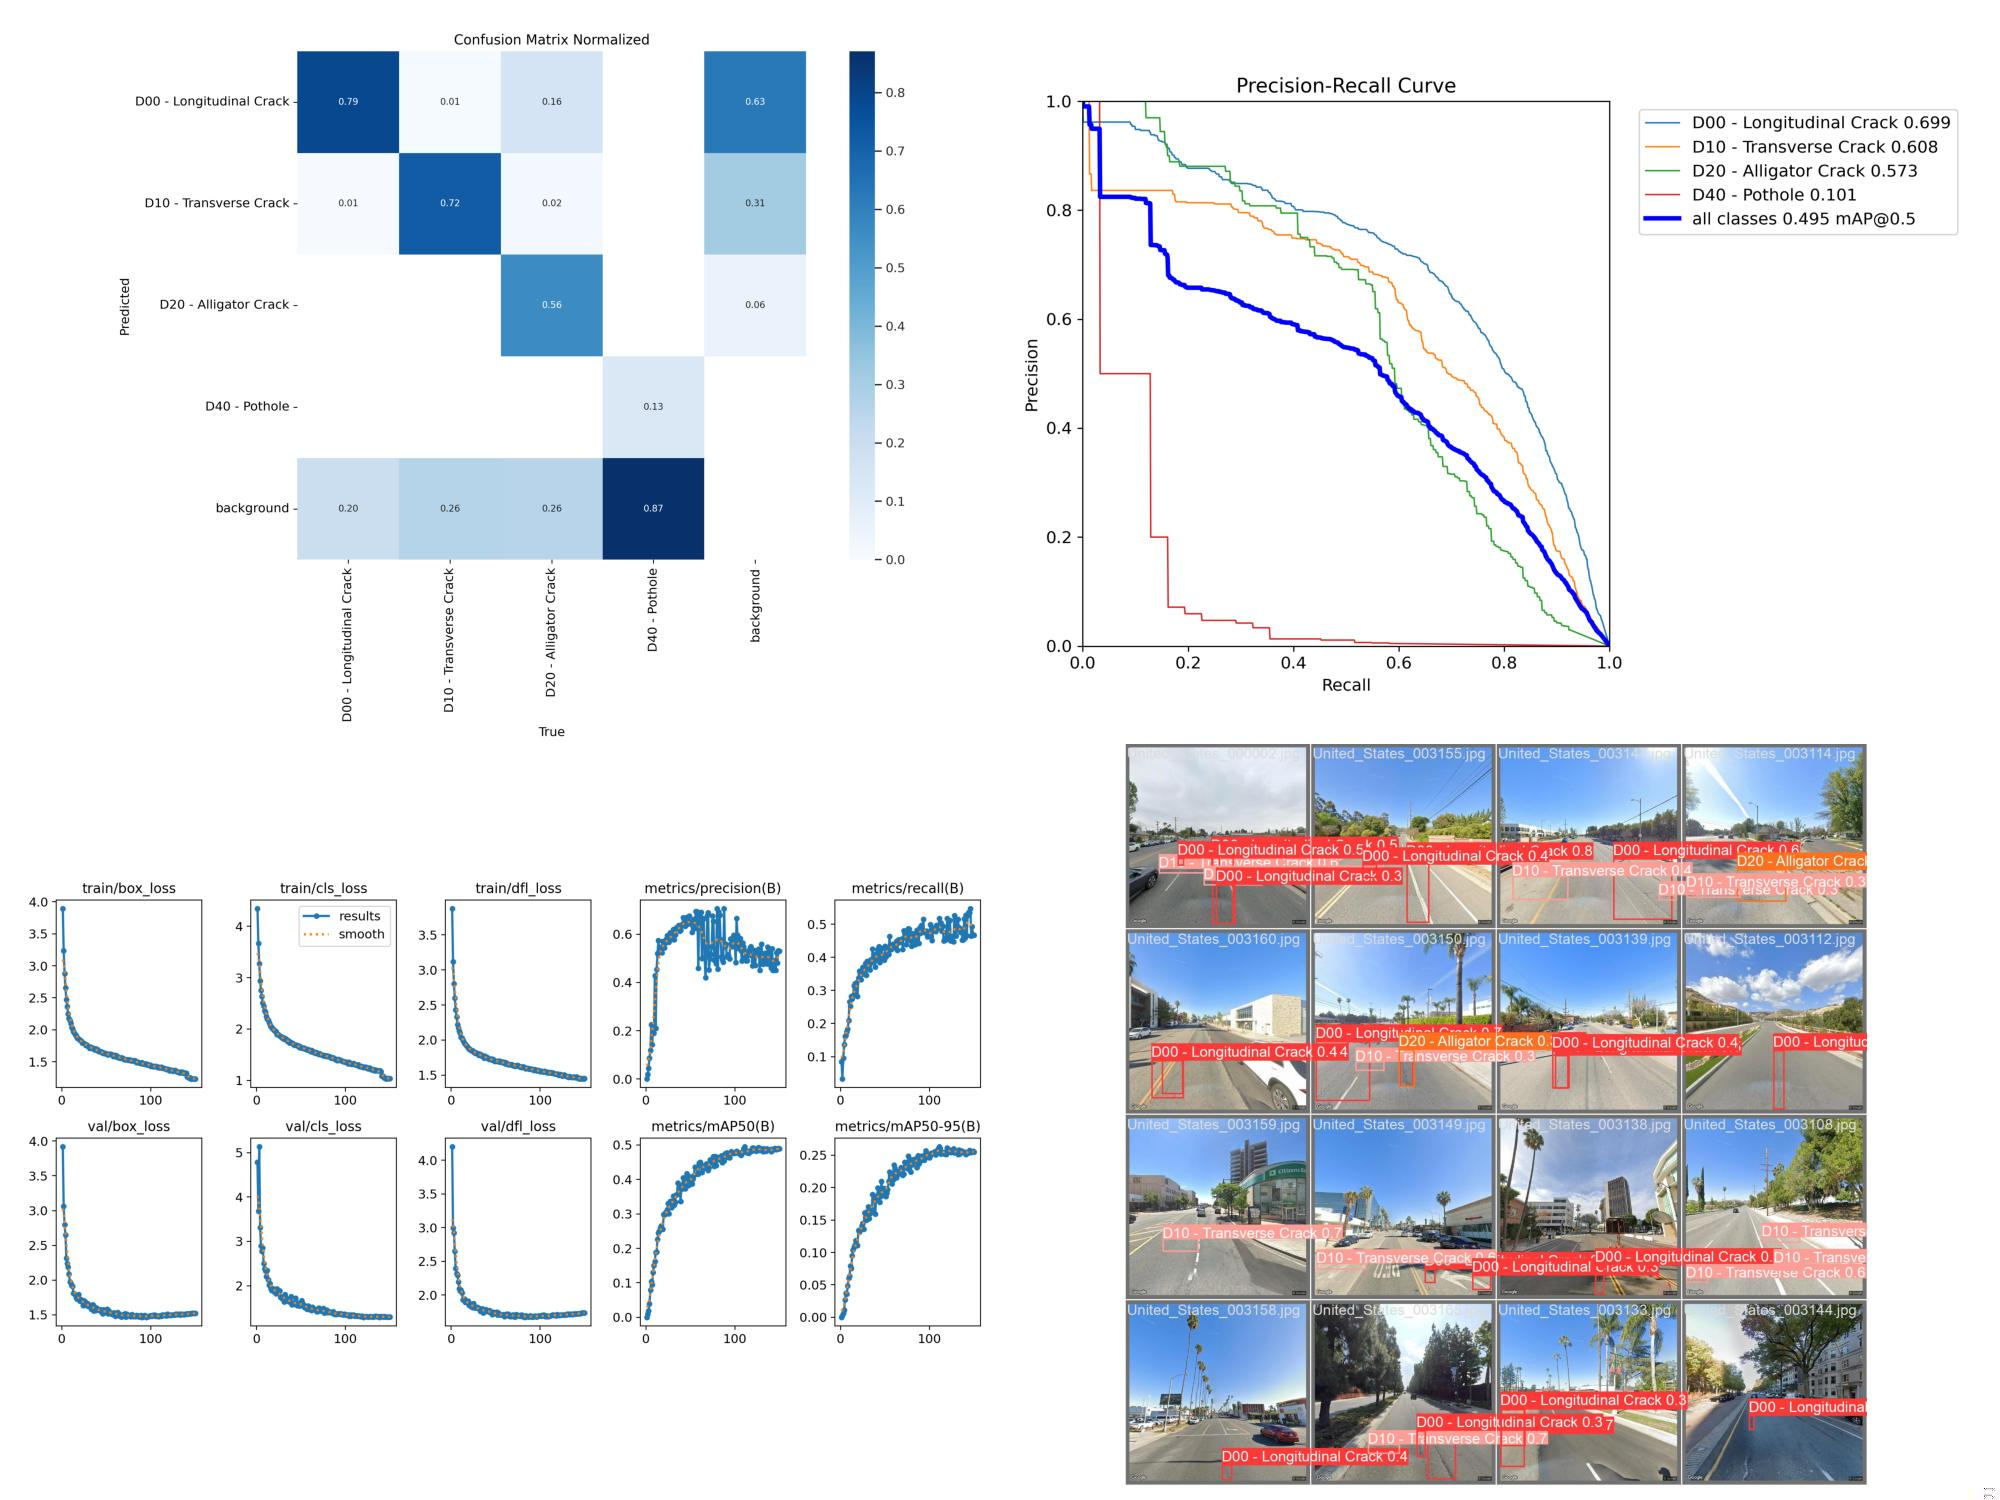
\includegraphics[width=0.9\textwidth]{graphs/metrics_grid.jpg}
    \caption{Ejemplos de gráficas de Ultralytics. De izquierda a derecha y de arriba a abajo: matriz de confusión, curva precision-recall, resultados de la evaluación y ejemplos de batch.}
    \label{fig:Ultralytics_metrics}
\end{figure}

